\section{Optimizations}
\label{sec:optimizations}


%\todo{check}

We apply four optimizations to the base algorithm to control intermediate blow‐up in the size of both the PN and the constructed semilinear set. 
%
An extensive empirical evaluation of these optimizations appears in Appendix~\ref{appendix:full_results}.

%\medskip
%\noindent
%\textbf{(1) Bidirectional slicing.} 
\subsection{Bidirectional slicing} 
When solving Petri net reachability, many places and transitions might be irrelevant to the specific target set~\cite{Ra12}.  
	We slice them before symbolic reasoning by combining forward and backward passes:  
	the forward pass over-approximates the places reachable from $M_0$; and symmetrically,   
	the backward pass traverses in reverse from any place that can influence a target constraint (hence over-approximating the places that can contribute to it).
	We iteratively remove non-forward-reachable and
	non-backward-relevant places and transitions, to a fixed point.  
	This process is illustrated in Fig.~\ref{fig:bidirectional_pruning}, and its soundness is proven in Theorem~\ref{thm:bidirectional-pruning}.




\begin{figure}[h]
	\centering
	
	% Top row: (a), (b)
	\begin{subfigure}[b]{0.45\textwidth}
		\centering
		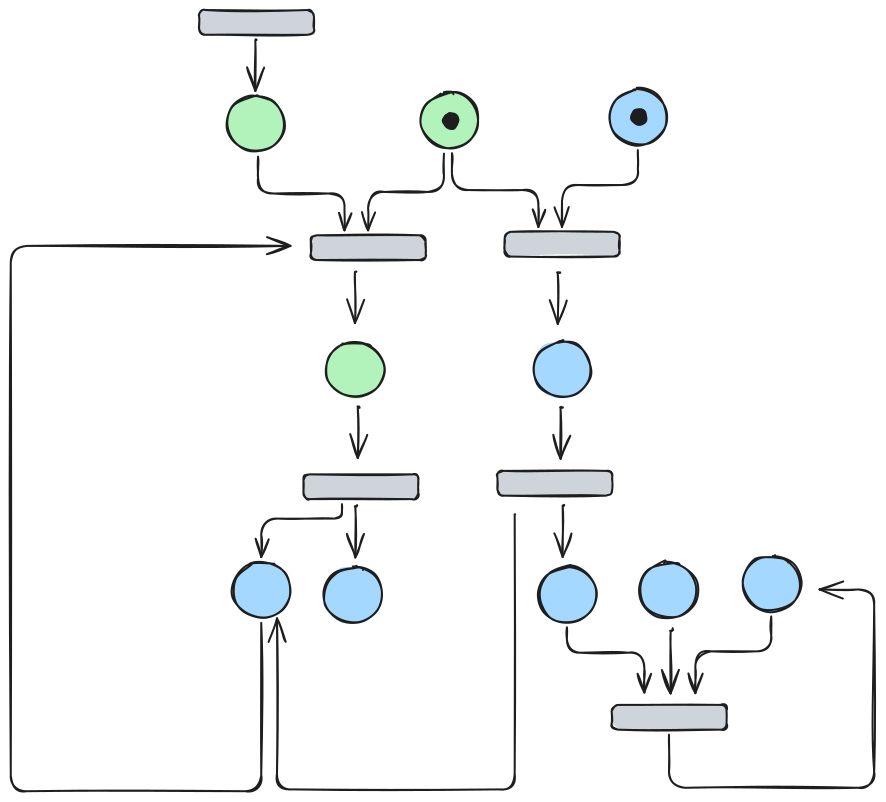
\includegraphics[width=\textwidth]{plots/bidirectional_pruning_step_a_updated.pdf}
		\caption{Step 0: initial Petri net, before slicing.}
		\label{fig:step:a}
	\end{subfigure}\hfill
	\begin{subfigure}[b]{0.45\textwidth}
		\centering
		\includegraphics[width=\textwidth]{plots/bidirectional_pruning_step_b_updated.pdf}
		\caption{Step 1: first forward pass.}
		\label{fig:step:b}
	\end{subfigure}
	
	\vspace{1em}
	
	% Bottom row: (c), (d), (e)
	\begin{subfigure}[b]{0.30\textwidth}
		\centering
		\includegraphics[width=\textwidth]{plots/bidirectional_pruning_step_c_updated.pdf}
		\caption{Step 2: first backward pass.}
		\label{fig:step:c}
	\end{subfigure}\hfill
	\begin{subfigure}[b]{0.23\textwidth}
		\centering
		\includegraphics[width=\textwidth]{plots/bidirectional_pruning_step_d_updated_2.pdf}
		\caption{Step 3: second forward pass.}
		\label{fig:step:d}
	\end{subfigure}\hfill
	\begin{subfigure}[b]{0.23\textwidth}
		\centering
		\includegraphics[width=\textwidth]{plots/bidirectional_pruning_step_e_updated_2.pdf}
		\caption{Step 4: final Petri net.}
		\label{fig:step:e}
	\end{subfigure}
	
	\caption{A Petri net during three rounds of bidirectional slicing: two forward passes and one backward pass. Black dots represent initial token markings; green places represent places that are allowed to be reachable in our constraints (i.e., aren't fixed to zero tokens in the final marking). Dashed shapes represent places and transitions that are identified as removable in the current iteration, and will be removed after it ends.}
	\label{fig:bidirectional_pruning}
\end{figure}


%\guy{check with mark (M0 projected on P or P'?)}

\begin{theorem}[Bidirectional Slicing Soundness]
	\label{thm:bidirectional-pruning}
	Let $N = (P, T, \Pre, \Post, M_0)$ be a Petri net and $S$ a target set.  
	Let $N' = (P',T',\,\Pre|_{P'\times T'},\,\Post|_{P'\times T'},\,M_0|_{P'})$ be the sliced net.  
	Then $S$ is reachable from $N$ iff it is reachable from $N'$.
\end{theorem}
%
%We depict this in Fig.~\ref{fig:bidirectional_pruning}, and prove Theorem~\ref{thm:bidirectional-pruning} in Appendix~\ref{appendix:BidirectionalProof}.
% (see the proof in Appendix~\ref{appendix:BidirectionalProof}).
%

% \medskip
% \noindent\textit{\textbf{Intuition.}}
% Before any heavy symbolic reasoning takes place, we apply bidirectional pruning on the underlying PN.  In the forward pass, we traverse from the initial marking to identify an over-approximation of all places and transitions that could ever fire; in the backward pass, we traverse backward from any place that can influence a target constraint, and identify over-approximations on transitions and places that cannot contribute to reaching it.  By iteratively repeating forward passes and backward passes until convergence, we remove every component of the net that cannot both originate and contribute to the reachable target set.  This dramatically shrinks the net in practice, often converting an intractably large model into one small enough for exhaustive analysis.

%\medskip
%\noindent
\subsection{Semilinear set pruning}  
A semilinear set $S=\bigcup_{i=1}^m L_i$ with 
	$L_i=\{\,\mathbf{b}_i+\sum_{\mathbf{p}\in P_i}n_p \mathbf{p} \mid n_p\in\mathbb N\}$ may contain redundant 
	period vectors or components.  
	Thus, during construction, we:
	(1) remove any period vector $\mathbf{p}\in P_i$ expressible as a nonnegative combination of $P_i\setminus\{\mathbf{p}\}$; 
	and (2) drop $L_i$ when $L_i\subseteq L_j$ (for \(i \neq j\)).  
	This pruning keeps formulas compact and solver calls tractable.




% it is common for some inequalities or disjuncts to add no new coverage beyond what other constraints already guarantee.  The redundant‐constraint elimination pass inspects each linear inequality and each disjunct in a disjunctive normal form, testing whether it is implied by the rest.  Any constraint or disjunct found redundant is dropped, ensuring that subsequent intersection, union, and projection operations work on the smallest necessary formula.  This streamlines the logic formula and prevents unnecessary size blow‐ups during solver invocations.

% %
% We replace each period‐basis \(P_i\) by
% \[
% P_i \;:=\;\{\,p\in P_i \mid p\notin\mathsf{Span}(P_i\setminus\{p\})\}
% \],
% Dropping any ``redundant'' periods, and removing any \(L_j\subseteq L_i\) for \(i\neq j\), iterating to a fixed point so no two components subsume one another.

%\medskip
%\noindent
\subsection{Generating fewer constraints}  
When computing the Parikh image of a regular expression as a semilinear set,
	most regex operations can be implemented without an exponential blow-up.
	However, the Kleene star is a notable exception. Given $S=\bigcup_{i=1}^m L_i$,  the Kleene closure $S^\ast$ can be expressed as a semilinear set by: 
	\[
	S^\ast=\bigcup_{I \subseteq \{1,...,m\}} 
	\Big\{\sum_{i \in I} \mathbf{b}_i + \sum_{\mathbf{p} \in \bigcup_{i \in I} (P_i\cup \{\mathbf{b}_i\})} n_p \mathbf{p}\Big\},
	\]
	yielding $2^m$ components. To mitigate this:
	(i) if $L_i=\{\mathbf{b}_i\}$ (period-less component), factor it out, star the rest, then add $\mathbf{b}_i$ as a period;  
	(ii) if $L_i=\{\sum_{\mathbf{p}\in P_i}n_p\mathbf{p}\}$ (zero base), likewise star the rest and add each $\mathbf{p}\in P_i$ as a period vector to the resulting set.  
	Each such case halves the component count and circumvents exponential blow-ups.




% Let $\mathrm{comp}(S)=\{L_1,\dots,L_m\}$ 
% be the multiset of linear components of the semilinear set 
% \(\displaystyle S=\bigcup_{i=1}^m L_i\), where each 
% \(\;L_i=b_i+\langle P_i\rangle\) with \(b_i\in\mathbb N^d\) and 
% \(P_i\subseteq\mathbb N^d\).  Define the pruning operator
% \[
% \mathrm{new}(\mathcal C)
% \;=\;
% \bigcup\bigl\{\,L\in\mathcal C \;\bigm|\;\nexists\,L'\in\mathcal C\setminus\{L\}:\;L'\subsetneq L\bigr\},
% \]
% which removes any component strictly containing another.  
% %
% \guy{Nicolas is it clear we mean that we fix their semilinear "meaning" of the regex operations? For example, + is union etc..}
% Then, we replace the naive semilinear‐set operations by
% \[
% S\;+\;T
% \;=\;
% \mathrm{new}\bigl(\mathrm{comp}(S)\,\cup\,\mathrm{comp}(T)\bigr),
% \]
% \[
% S\;\cdot\;T
% \;=\;
% \mathrm{new}\Bigl(\{\,L_i\cdot L'_j \mid L_i\in\mathrm{comp}(S),\;L'_j\in\mathrm{comp}(T)\}\Bigr),
% \]
% where for
% \(\;L_i=b_i+\langle P_i\rangle,\;L'_j=b'_j+\langle P'_j\rangle\) we set
% $
% L_i\cdot L'_j
% =\;(b_i+b'_j)\;+\;\langle\,P_i\cup P'_j\,\rangle.
% $
% Finally, for Kleene‐star and plus on the regex side one similarly applies
% \(\mathrm{new}(\cdot)\) to the collection of ``folded” components instead of
% building all intermediate ones:
% \[
% S^*
% =\mathrm{new}\Bigl(\bigcup_{k\ge0}\bigl(\mathrm{comp}(S)\bigr)^k\Bigr),
% \qquad
% S^+
% =S\cdot S^*.
% \]

% \medskip
% \noindent\textit{\textbf{Intuition.}}
% %
% During set construction --- especially when introducing new existentially‐quantified variables or combining transition effects, we selectively avoid generating any marking that would strictly dominate an already‐seen solution.  In effect, whenever a candidate disjunct would yield a superset of an existing one, it is skipped entirely.  This ``generate‐less” heuristic stops the proliferation of large, overlapping regions in the semilinear description.  In benchmarks with large state spaces, it can reduce the number of intermediate branches by orders of magnitude.

%\medskip
%\noindent
\subsection{Strategic Kleene elimination order} 
%
We use \textit{Kleene's algorithm}~\cite{Kl56} to translate the serializability NFA into a regex.
% 
The size of the generated semilinear set is not only impacted by how the
	semilinear set operations are implemented, but also by what \textit{specific} regular
	expression is given as input: a single regular language may be represented by a
	number of equivalent regexes, each of different complexity.
	%
	In particular, as Kleene star can cause a large blow-up in the semilinear set size,
	we are especially sensitive to the \emph{star height} of the generated regex.
	%
	Naive Kleene elimination may introduce many nested stars.  
	We reduce this by strategically choosing to eliminate lower-degree states first:
	\[
	q^*=\arg\min_{q\in Q}\bigl(|\delta^A_{\mathrm{in}}(q)|+|\delta^A_{\mathrm{out}}(q)|\bigr).
	\]
	 
	
	\smallskip
	\noindent
	As we demonstrate in Appendix~\ref{appendix:full_results}, our optimizations expedite the search procedure and make the representations \textit{significantly} more compact. This, in turn, enables deciding serializability for instances that are otherwise intractable.


%\medskip
%\noindent
%\textbf{(4) Strategic Kleene elimination order.}  
%The size of the generated semilinear set is not only impacted by how the
%semilinear set operations are implemented, but also by what specific regular
%expression is given as input: a single regular language may be represented by a
%number of equivalent regexes, each of different complexity.
%%
%In particular, as Kleene star can cause a large blow-up in the semilinear set size,
%we are especially sensitive to the \emph{star height} of the generated regex.
%%
%We use Kleene's algorithm to convert an NFA $\mathcal A=(Q,\Sigma,\delta,q_0,F)$ to a regex, which works by repeated state elimination, choosing one state at a time.
%Naively, when eliminating states in an arbitrary order, Kleene's algorithm may generate regexes with a much greater star height than necessary---a problem
%when converting to semilinear sets.
%%
%Therefore, we heuristically optimize the state elimination order to end up with a smaller regex. Formally, we pick the next state:
%\[
%q^* = 
%\arg\min_{q\in Q'}\bigl(|\delta_{\mathrm{in}}(q)|+|\delta_{\mathrm{out}}(q)|\bigr)
%\]
%where \(Q'\subseteq Q\) are the states remaining to be eliminated, choosing to
%eliminate states with a smaller total degree first.
%%
%This empirically keeps the resulting regexes small.

% \medskip
% \noindent\textit{\textbf{Intuition.}}
% When converting an NFA to a single regex, we pick the next state to eliminate by heuristically choosing the  state with the fewest incoming and outgoing edges.
% This optimization allows for circumventing 
% overblown expressions resulting in naive translations, especially with regard to  Kleene closures (the “\(\mathsf{*}\)” operator).  Instead, we analyze the structure of sub-expressions under the various operators --- estimating their branching factor, and reordering them so that simpler, low‐branching components are expanded first.  
%This adaptive ordering often leads to early detection of fixed points or dead‐ends, preventing the combinatorial explosion that arises when complex loops are expanded prematurely.  
